% !TeX program = xelatex
\documentclass[9pt]{beamer}
\usepackage{xcolor}
\definecolor{orange}{HTML}{F67941}
\definecolor{red}{HTML}{AC454A}
\definecolor{brown}{HTML}{EAD296}
\definecolor{darkgrey}{HTML}{313630}
\usefonttheme{professionalfonts} % using non standard fonts for beamer
\usefonttheme{serif} % default family is serif
\usepackage{fontspec}
\usepackage{natbib}
%\usepackage[T1]{fontenc}

\bibliographystyle{abbrv}
%\setmainfont{Liberation Serif}
%\setmainfont{Liberation Serif}
\setmainfont{Comfortaa}
%\usepackage[T1]{fontenc}

\setbeamercolor{frametitle}{bg=orange,fg=white}
\setbeamercolor{author in head/foot}{bg=orange,fg=white}



%\setbeamertemplate{itemize items}[circle]
\useinnertheme{circles}
\setbeamercolor{palette primary}{bg=orange,fg=white}
%\setbeamercolor{palette secondary}{bg=red,fg=white}
\setbeamertemplate{itemize item}{\color{darkgrey}$\circ$}
\setbeamercolor{structure}{fg=red} % itemize, enumerate, etc

%\setbeamercolor{section in head/foot}{bg=red}
\setbeamercolor{title}{fg=orange} %, bg=brown
\setbeamercolor{author}{fg=darkgrey}
\setbeamercolor{institute}{fg=darkgrey}
\setbeamercolor{date}{fg=darkgrey}
%\setbeamercolor{normal text}{fg=darkgrey}
\makeatletter
\setbeamertemplate{headline}{%
	\usebeamercolor[bg]{frametitle}\rule{\textwidth}{1cm}
}
\setbeamerfont{title}{size=\LARGE}
\setbeamerfont{institute}{size=\normalsize}
\renewcommand*{\bibfont}{\scriptsize}


\setbeamertemplate{frametitle}{%
	\vskip-1cm%
	\begin{minipage}[c][\headheight][c]{\textwidth}%
		\usebeamerfont{frametitle}%
		\strut\insertframetitle\par
		{%
			\ifx\insertframesubtitle\@empty%
			\else%
			{\usebeamerfont{framesubtitle}\usebeamercolor[fg]{framesubtitle}\strut\insertframesubtitle\par}%
			\fi
		}%      
		\vspace*{-0.1cm}
	\end{minipage}%
	\vskip-0.1em
}
%\setbeamertemplate{footline}{%
%	\leavevmode%
%	\hbox{\begin{beamercolorbox}[wd=\paperwidth,ht=4.5ex,dp=3.125ex]{author in head/foot}%
%			\usebeamerfont{author in head/foot} bar
%	\end{beamercolorbox}}%
%	\vskip0pt%
%}
\makeatother

\title{Uncertainty in\\Recurrent Decision Tree Classifiers}
\author{Stefan Wezel}
\institute{Explainable Machine Learning}
\date{\today}

\begin{document}

\setbeamercolor{background canvas}{bg=white}
\setbeamercolor{normal text}{fg=darkgrey}
\usebeamercolor[fg]{normal text}
\begin{frame}[plain]
	\titlepage
\end{frame} 

\setbeamercolor{background canvas}{bg=white}
\setbeamercolor{normal text}{fg=darkgrey}
\usebeamercolor[fg]{normal text}
\setbeamertemplate{itemize item}{\color{darkgrey}$\circ$}
\begin{frame}
\frametitle{What?}
\framesubtitle{Setting}
	\begin{itemize}\setlength\itemsep{1em}
	\item There are a lot of architectures that perform great on image classification tasks
	\item Maybe, most prominently: ResNet
	\item However, they only yield a classification
	\item In many settings a classification is not worth much without the reasoning behind it
	\end{itemize}
\end{frame} 


\setbeamercolor{background canvas}{bg=white}
\setbeamercolor{normal text}{fg=darkgrey}
\usebeamercolor[fg]{normal text}
\setbeamertemplate{itemize item}{\color{darkgrey}$\circ$}
\begin{frame}
\frametitle{What?}
\framesubtitle{Recap}
	\begin{figure}
	\centering
	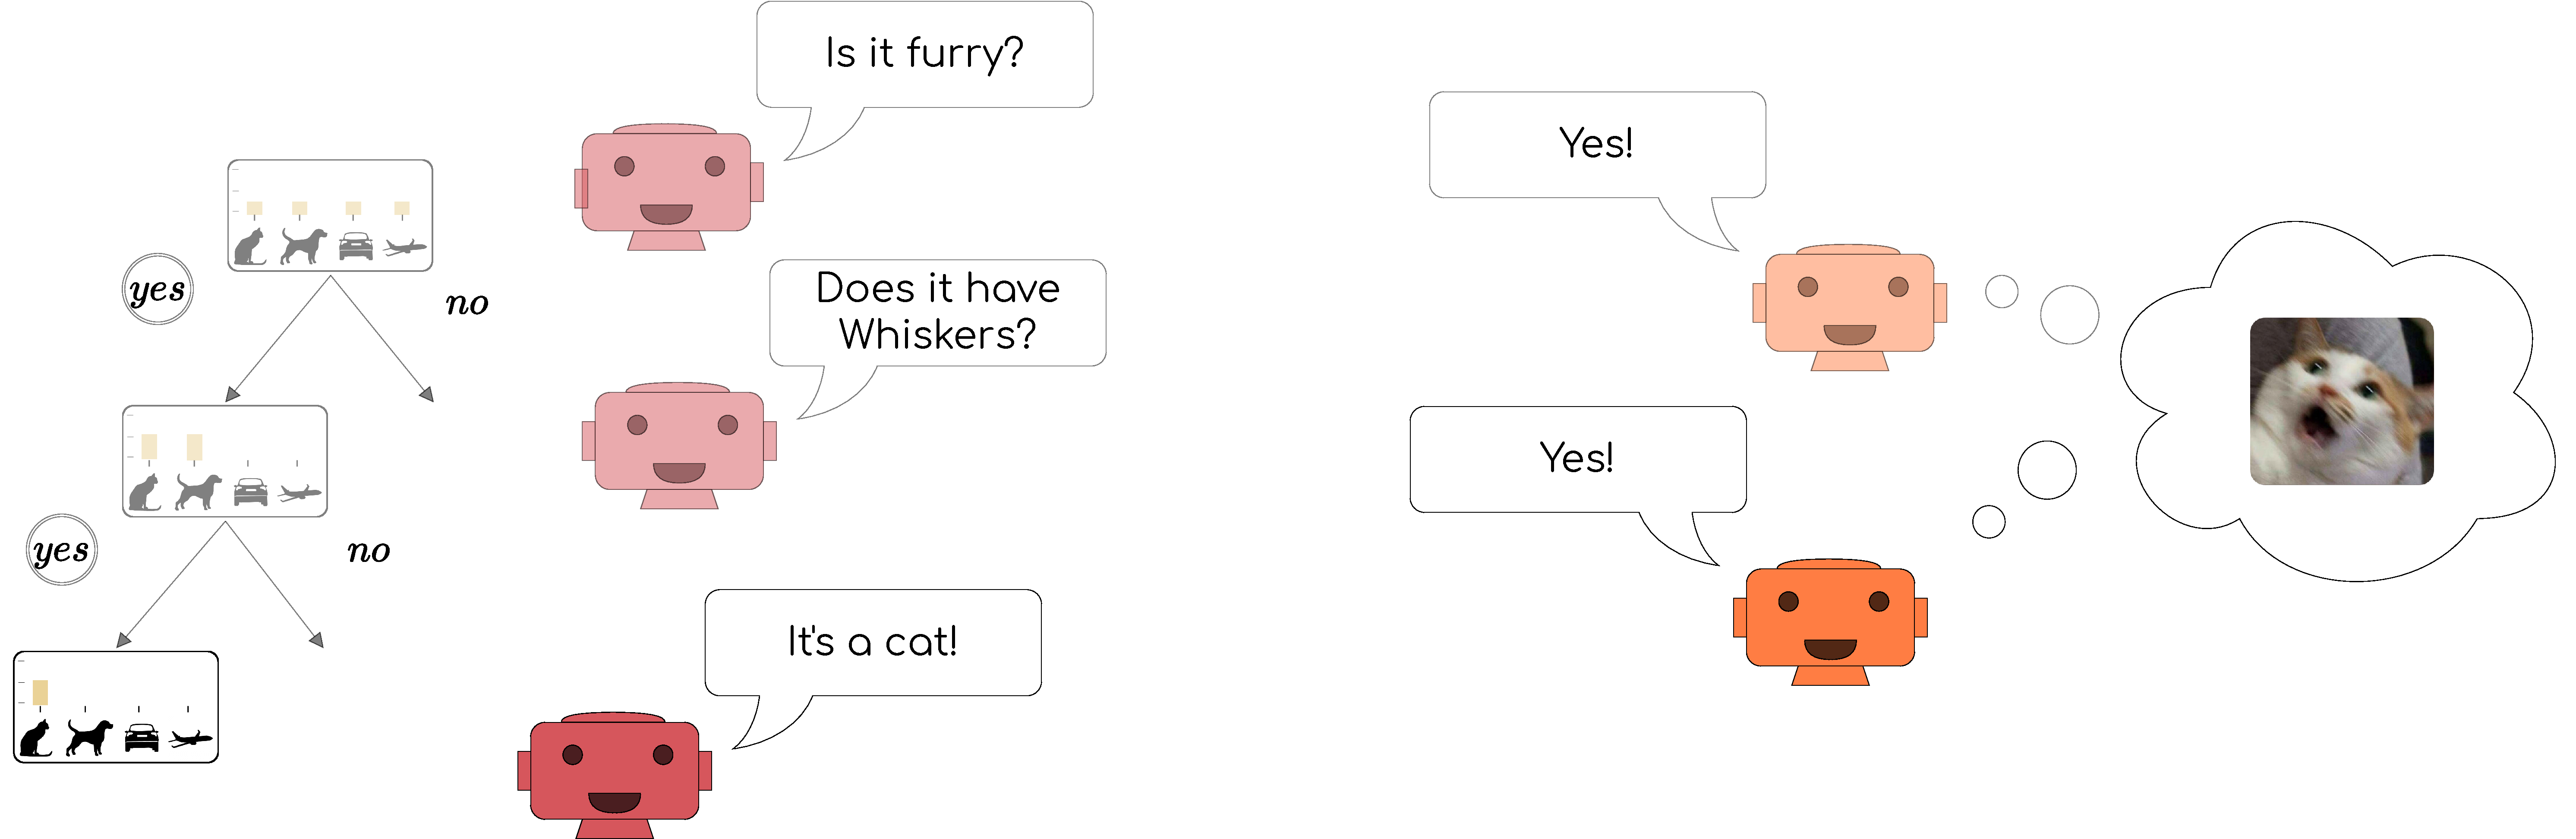
\includegraphics[width=1\textwidth]{images/rdtc_intuition.pdf}
	%\caption[caption for ]{After collecting images of birds, the ornithologist lets our proposed model classify the vast amount of data. Only in cases of high uncertainty, she is consulted and can classify the image manually. \footnotemark}
	%\label{fig:qual}
\end{figure}
\begin{itemize}\setlength\itemsep{1em}
	\item Two agents
	\item One is asking questions and one is answering them
	\item The unfolding decision process is an interpretable tree
\end{itemize}
\end{frame} 


\setbeamercolor{background canvas}{bg=white}
\setbeamercolor{normal text}{fg=darkgrey}
\usebeamercolor[fg]{normal text}
\setbeamertemplate{itemize item}{\color{darkgrey}$\circ$}	
\begin{frame}
\frametitle{What?}
\framesubtitle{Recap}
\begin{figure}
	\centering
	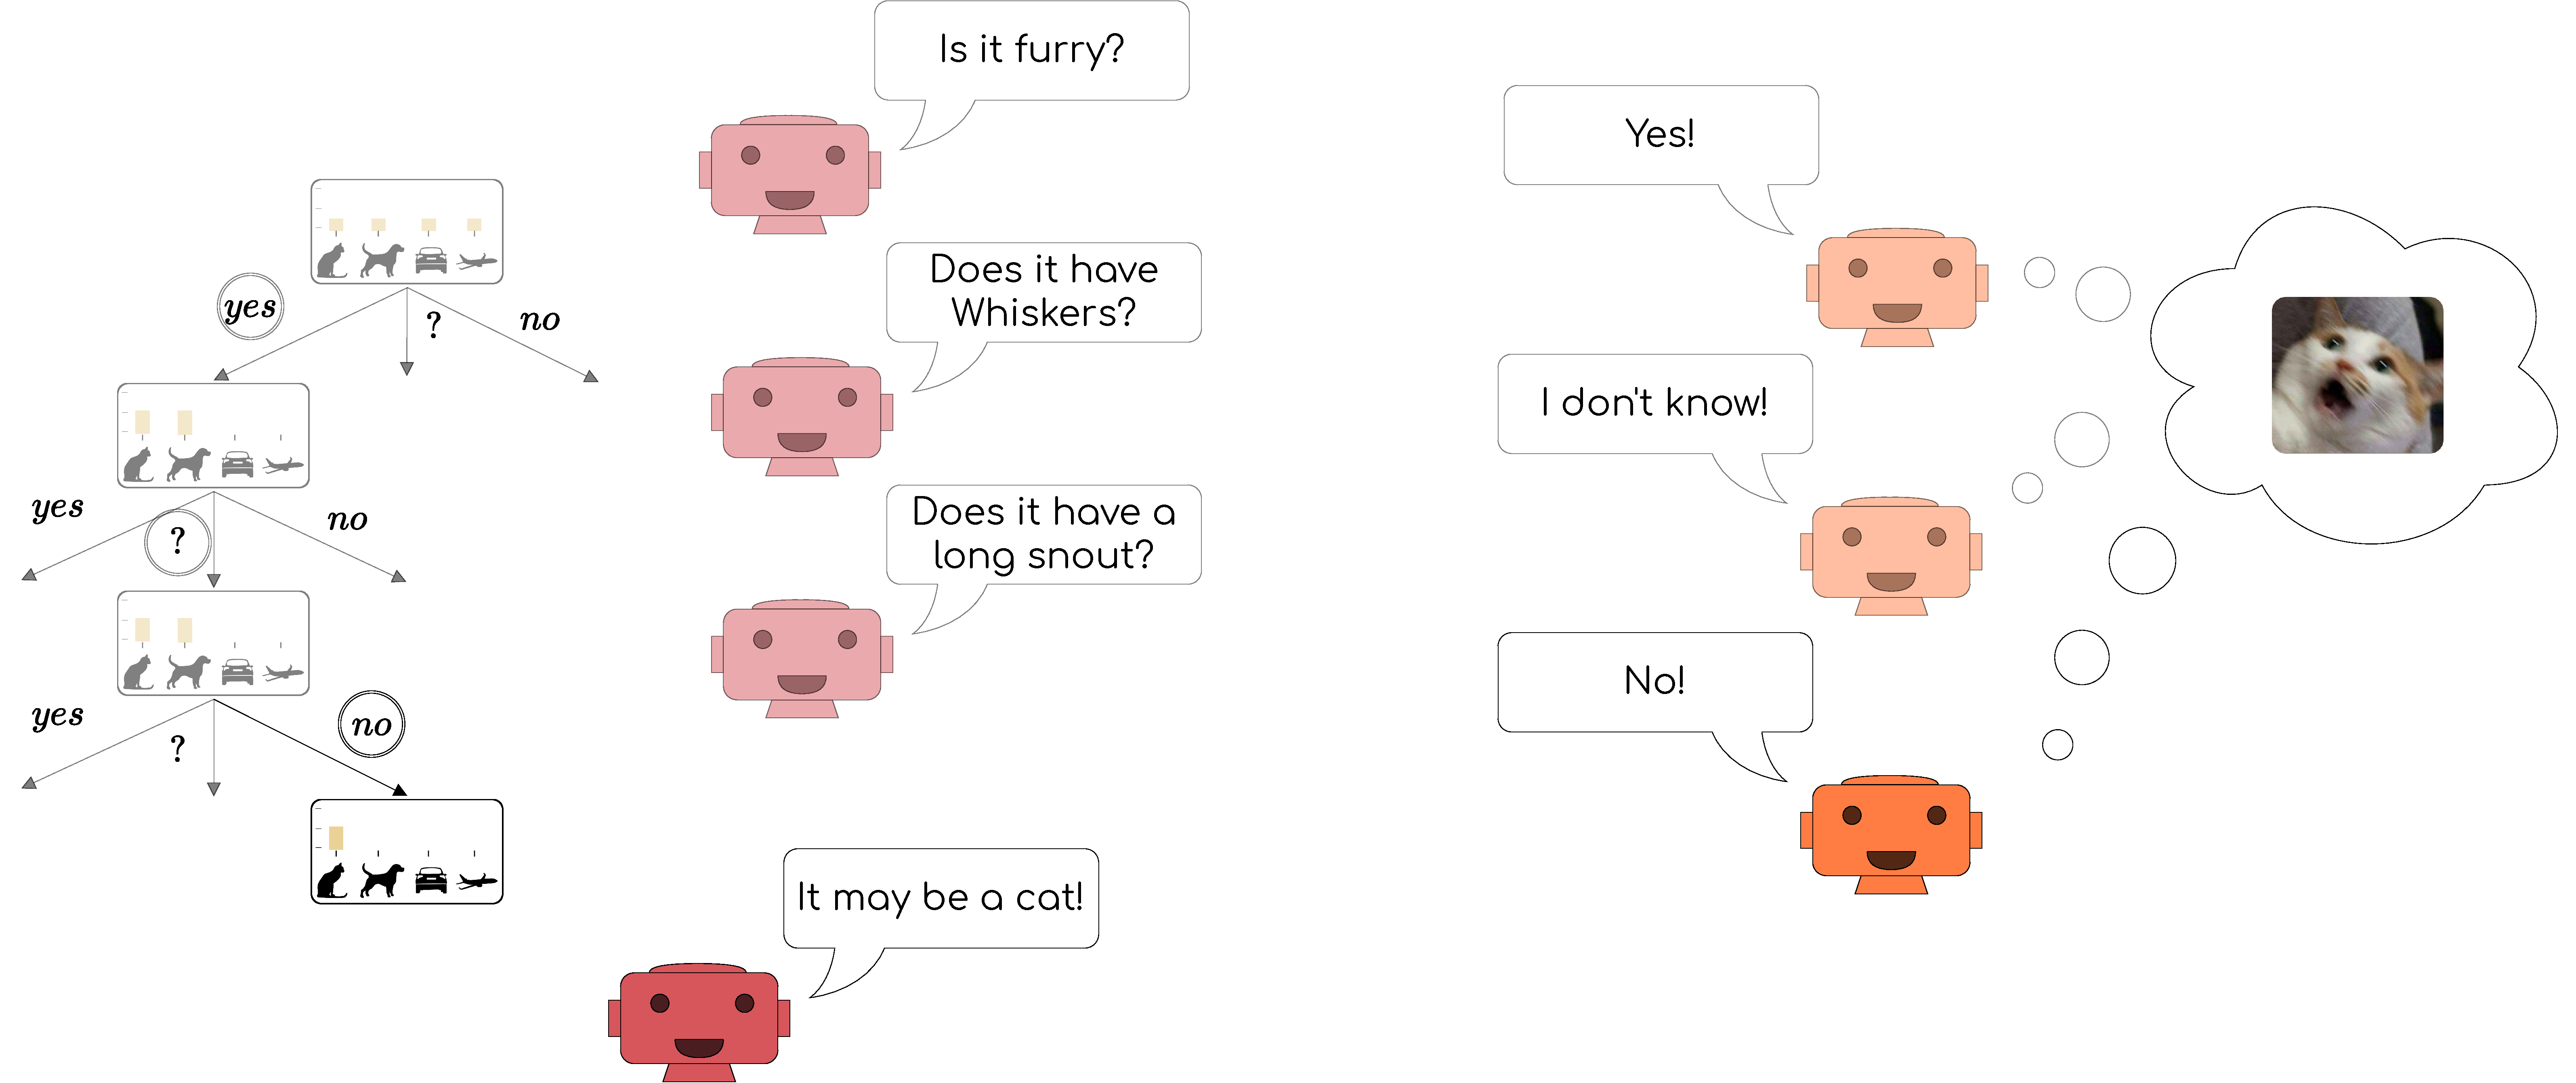
\includegraphics[width=1\textwidth]{images/urdtc_intuition.pdf}
	%\caption[caption for ]{After collecting images of birds, the ornithologist lets our proposed model classify the vast amount of data. Only in cases of high uncertainty, she is consulted and can classify the image manually. \footnotemark}
	%\label{fig:qual}
\end{figure}
\begin{itemize}\setlength\itemsep{1em}
	\item Two agents
	\item One is asking questions and one is answering them
	\item The unfolding decision process is an interpretable tree
\end{itemize}
\end{frame} 



\setbeamercolor{background canvas}{bg=white}
\setbeamercolor{normal text}{fg=darkgrey}
\usebeamercolor[fg]{normal text}
\setbeamertemplate{itemize item}{\color{darkgrey}$\circ$}
\begin{frame}
\frametitle{Why do we need uncertainty?}
\framesubtitle{A Practical Example...}
	\begin{figure}
		\centering
		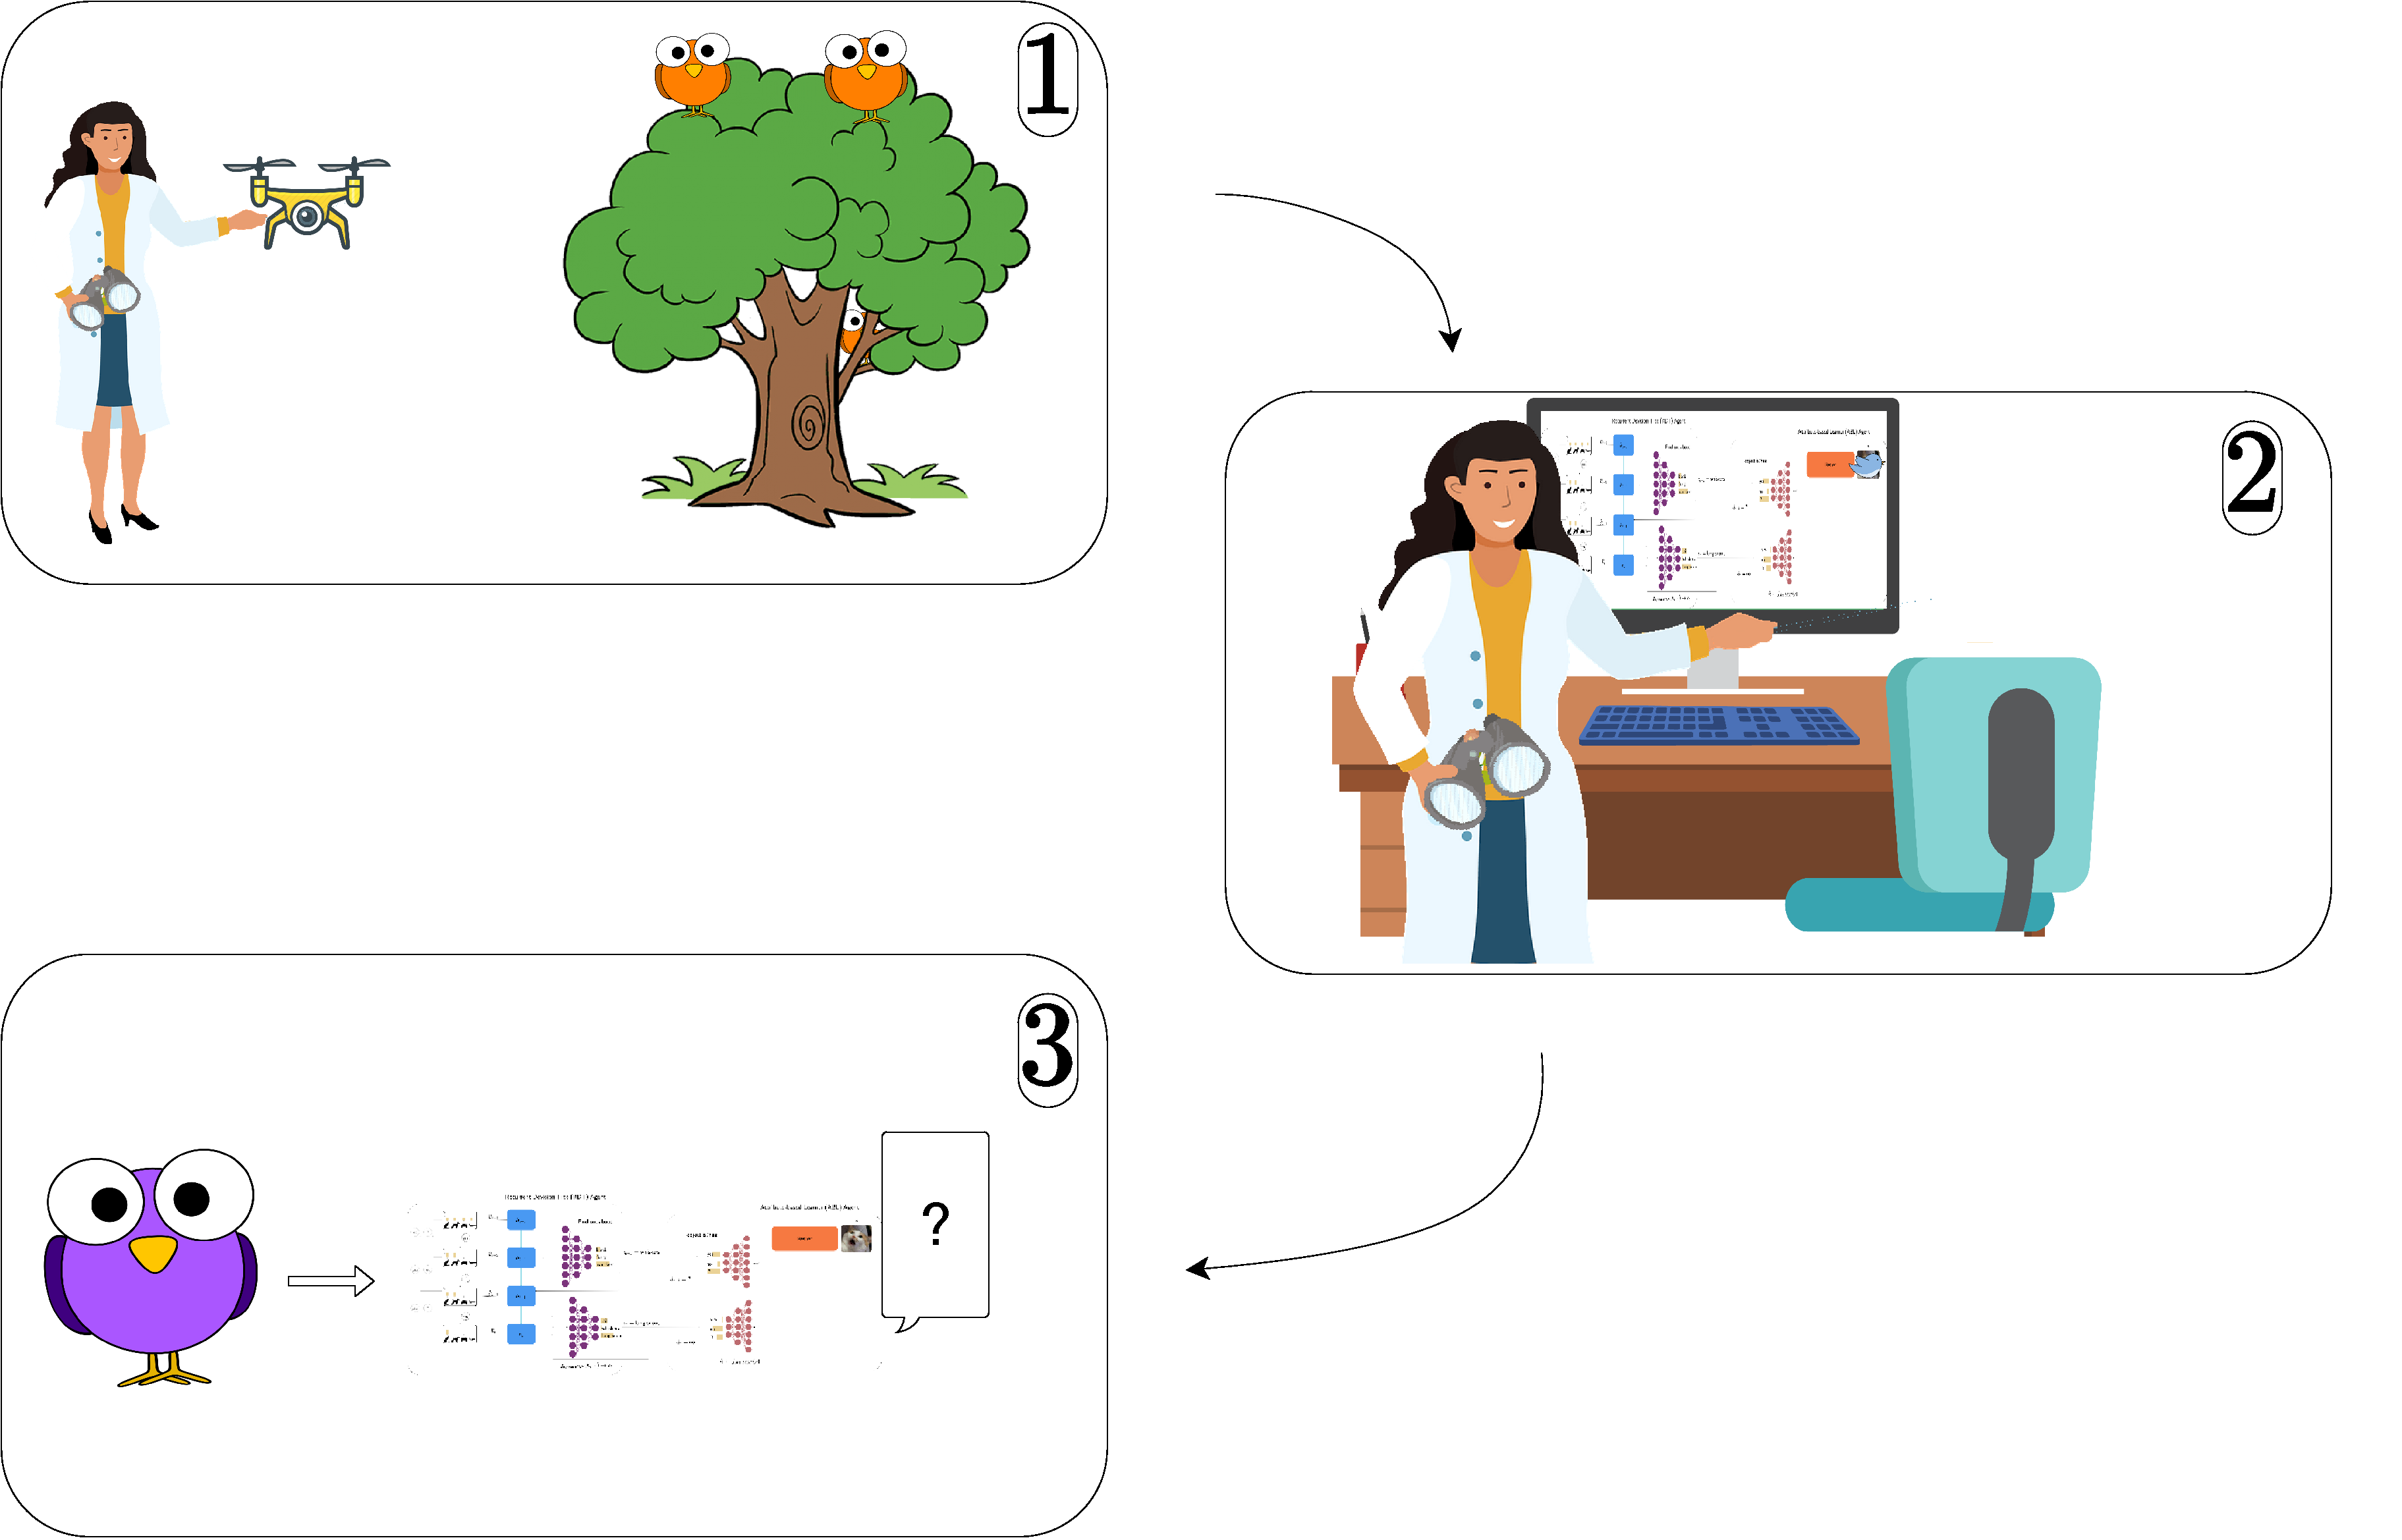
\includegraphics[width=0.6\textwidth]{images/ornithology.pdf}
		%\caption[caption for ]{After collecting images of birds, the ornithologist lets our proposed model classify the vast amount of data. Only in cases of high uncertainty, she is consulted and can classify the image manually. \footnotemark}
		%\label{fig:qual}
	\end{figure}
	\begin{itemize}\setlength\itemsep{1em}
	\item The ornithologist is tasked to survey bird species, which she automates using a drone and computer vision software
	\item She uses our model to go through the vast amount of collected data
	\item Some bird species unknown to the model appear in the data. The model yields high uncertainty and the ornithologist can classify them manually
	\end{itemize}
\end{frame}

\setbeamercolor{background canvas}{bg=orange}
\setbeamercolor{normal text}{fg=white}	
\usebeamercolor[fg]{normal text}
\setbeamertemplate{itemize item}{\color{white}$\circ$}
\begin{frame}[plain]
\begin{itemize}
	\item The RDTC model yields a decision tree as explaination, revealing the reasoning behind a classification
	\item Uncertainty allows the model to detect OOD examples
	\item This is useful in settings where high-risk decision can be dangerous
\end{itemize}
\end{frame}
%\setbeamertemplate{background canvas}{bg=white}



\setbeamercolor{background canvas}{bg=white}
\setbeamercolor{normal text}{fg=darkgrey}
\usebeamercolor[fg]{normal text}
\setbeamertemplate{itemize item}{\color{darkgrey}$\circ$}
\begin{frame}
\frametitle{How?}
\framesubtitle{Architecture}
\begin{figure}
	\centering
	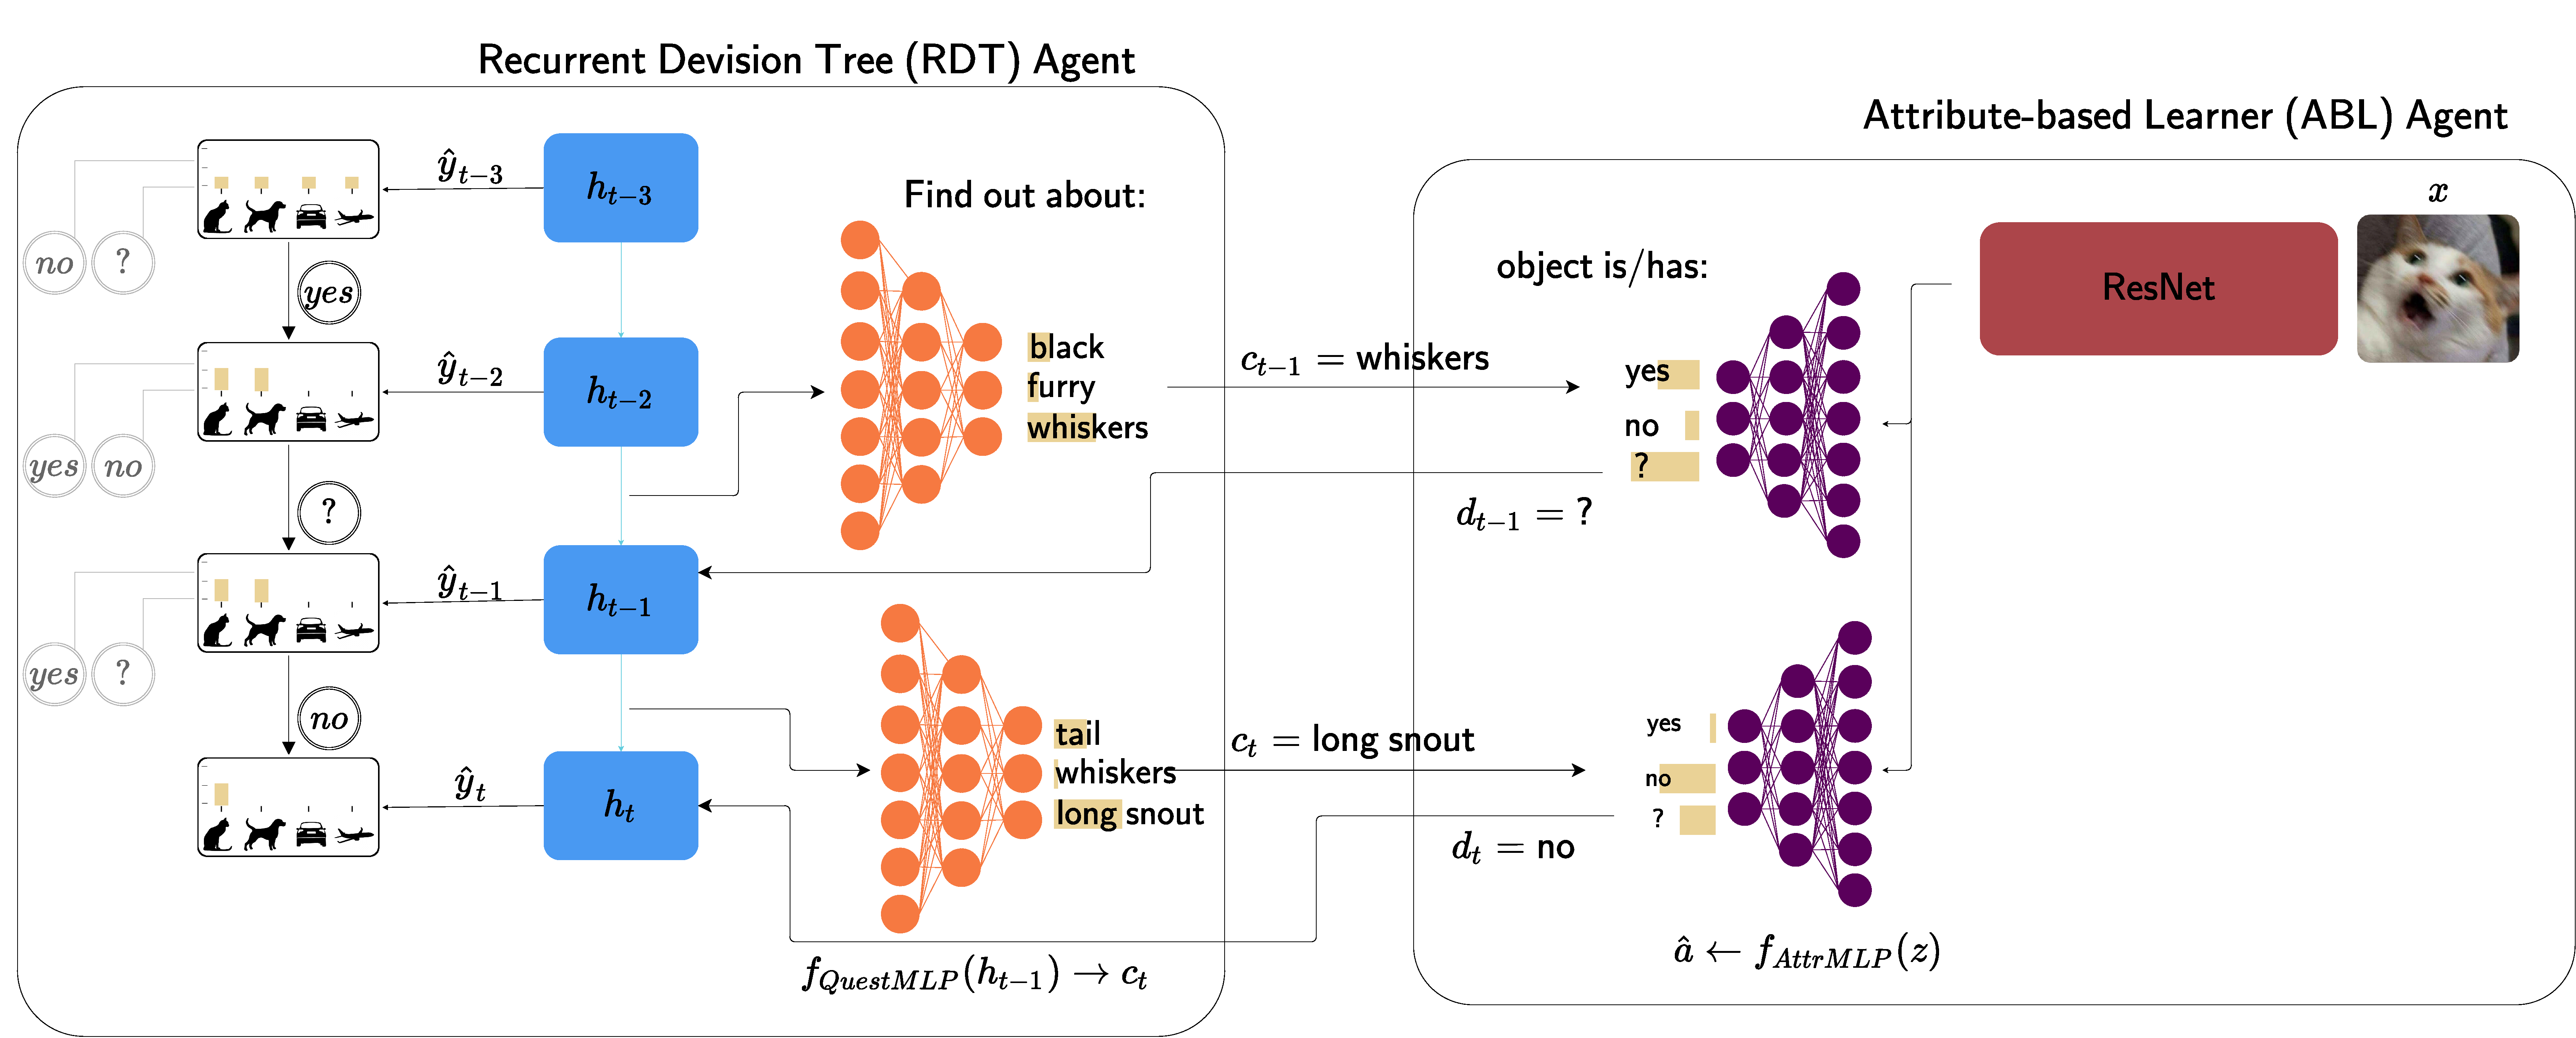
\includegraphics[width=0.9\textwidth]{images/uncertaintRDTC.pdf} 
	%\caption{The RDT asks questions about presence, absence or uncertainty of attributes. The answers, given by the AbL are used by the RDT agent to make a classification each iteration.}
	\label{fig:uncertainRDTC}
\end{figure}
\begin{itemize}
	\item The RDT can not see the images but only ask whether an attribute is present in the image
	\item The AbL can see the image and based on features answer the RDT's questions
\end{itemize}
\end{frame} 





%AbL
\setbeamercolor{background canvas}{bg=white}
\setbeamercolor{normal text}{fg=darkgrey}
\usebeamercolor[fg]{normal text}
\setbeamertemplate{itemize item}{\color{darkgrey}$\circ$}
\begin{frame}
\frametitle{Attribute-based Learner}
\framesubtitle{Answering questions}
\begin{itemize}
	\item We extract features from a given image using a ResNet
	\item A MLP maps extracted features to 'yes-no' answers indicating absence/presence of attributes
	\item It returns a tensor with the of shape number of attributes $\times$ decision size
	\item We get a discrete answer from our AbL though applying \begin{align*}
	&TempSoftmax(log\;\pi) = \frac{exp((log\;\pi_i)/\tau)}{\sum_{j=1}^{K}exp((log\;\pi_j)/\tau)} = d_t
	\text{ on }
	log\;\pi \\
	&\text{ which are the logit values for either 'Yes', or 'No' per attribute.}
\end{align*}
\item The TempSoftmax serves as differentiable approximation to a one argmax returning a one-hot encoding
\end{itemize}
\end{frame}


%RDT
\setbeamercolor{background canvas}{bg=white}
\setbeamercolor{normal text}{fg=darkgrey}
\usebeamercolor[fg]{normal text}
\setbeamertemplate{itemize item}{\color{darkgrey}$\circ$}	
\begin{frame}
\frametitle{Recurrent Decision Tree}
\framesubtitle{Building a decision tree}
\begin{itemize}
%	\item The RDT consists of several models:
		\item LSTM
		\begin{itemize}
			\item Hidden state based on previous hidden states and new answers
		\end{itemize}
		\item Explicit Memory
		\begin{itemize}
			\item Stores all questions and corresponding answers
			\item This is our decision tree
		\end{itemize}
		\item $f_{ClassMLP}$
		\begin{itemize}
			\item Make classification based on LSTM's hidden state
		\end{itemize}
		\item $f_{QuestMLP}$
		\begin{itemize}
			\item Find next question to ask based on LSTM's hidden state
			\item Next question is the index the $f_{QuestMLP}$ poses
			\item To turn logits into a discrete value, Gumbel softmax is used
			\item This allows us to sample from a categorical distribution
			\item \begin{align*}
				GumbelSoftmax(log\;\pi) &= \frac{exp((log\;\pi_i + g_i)/\tau)}{\sum_{j=1}^{K}exp((log\;\pi_j + g_j)/\tau)}
			\end{align*}
		\end{itemize}
		
\end{itemize}
\end{frame}


% Trianing
\setbeamercolor{background canvas}{bg=white}
\setbeamercolor{normal text}{fg=darkgrey}
\usebeamercolor[fg]{normal text}
\setbeamertemplate{itemize item}{\color{darkgrey}$\circ$}	
\begin{frame}
\frametitle{Training}
\framesubtitle{the two agents}
\begin{itemize}
	\item We optimize for class and attribute accuracy
	\item \begin{align*}
	\mathcal{L} = \frac{1}{T}\sum_{t=1}^{T}\left[(1-\lambda)\mathcal{L}_{CE}(y,\hat{y}_t) + \lambda \mathcal{L}_{CE}(\alpha_{y,c_t},\hat{\alpha}_{c_t}) \right]
	\end{align*}
	\item $\lambda$ can be used to balance the two loss terms
	\item For all of our experiments, we use $\lambda=0.2$
\end{itemize}
\end{frame}



\setbeamercolor{background canvas}{bg=orange}
\setbeamercolor{normal text}{fg=white}	
\usebeamercolor[fg]{normal text}
\setbeamertemplate{itemize item}{\color{white}$\circ$}
\begin{frame}[plain]
\begin{itemize}
	\item The RDTC is a model consisting of two agents
	\item The RDT agent can not see the data but can ask questions whether certain attributes are present
	\item The AbL can see the data and can answer the RDT's questions
\end{itemize}
\end{frame}
%\setbeamertemplate{background canvas}{bg=default}







% Related Work
\setbeamercolor{background canvas}{bg=white}
\setbeamercolor{normal text}{fg=darkgrey}
\usebeamercolor[fg]{normal text}
\setbeamertemplate{itemize item}{\color{darkgrey}$\circ$}	
\begin{frame}
\frametitle{Background}
\framesubtitle{A small excursion to Gaussian Processes (GP)}
\begin{figure}
	\centering
	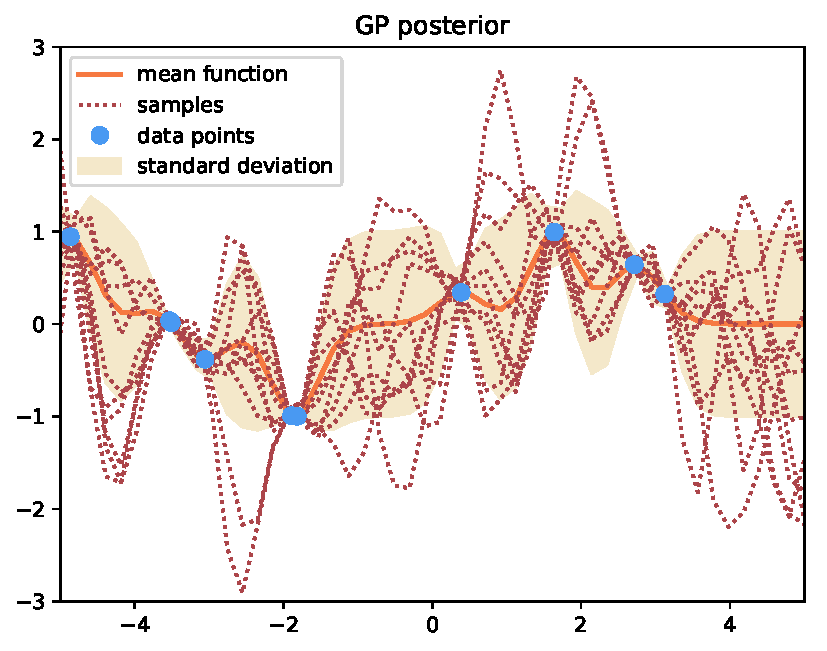
\includegraphics[width=0.6\textwidth]{images/post.pdf}
	\begin{itemize}
		\item Data points can be described by (infinitely) many functions
		\item A GP is a PDF over these functions
		\item Intuition: $\rightarrow$ a GP yields a probability for function values at any given index
		\item Parameterized by mean function and covariance function
		\item The variance resembles the model uncertainty where no data is given
	\end{itemize}
	%\caption{Correlations between misclassification rate, uncertainty, and usage of attributes.}
	%\label{fig:corr_matrix}
\end{figure}
\end{frame}


\begin{frame}
\setbeamercolor{background canvas}{bg=white}
\setbeamercolor{normal text}{fg=darkgrey}
\usebeamercolor[fg]{normal text}
\setbeamertemplate{itemize item}{\color{darkgrey}$\circ$}	
\frametitle{Background}
\framesubtitle{Dropout Uncertainty Estimation}
	\begin{itemize}
	\item A GP can be seen as an infinitely wide neural network
	\item In turn, we can view a neural network with a finite amount of layers as an approximation to a GP
	\item To compute the posterior in GP's, methods of variational inference are used
	\begin{itemize}
		\item GP objective gets turned into a minimization objective
		\item For computing covariance matrix, we use Monte-Carlo integration
	\end{itemize}
	\item This allows us to rewrite a GP's objective as to objective of a dropout neural network
	\item This in turn allows us to retrieve uncertainty estimates from dropout neural nets
\end{itemize}
\end{frame}




\setbeamercolor{background canvas}{bg=white}
\setbeamercolor{normal text}{fg=darkgrey}
\usebeamercolor[fg]{normal text}
\setbeamertemplate{itemize item}{\color{darkgrey}$\circ$}
\begin{frame}
\frametitle{How?}
\framesubtitle{Do we get uncertainty information?}\begin{figure}
	\centering
	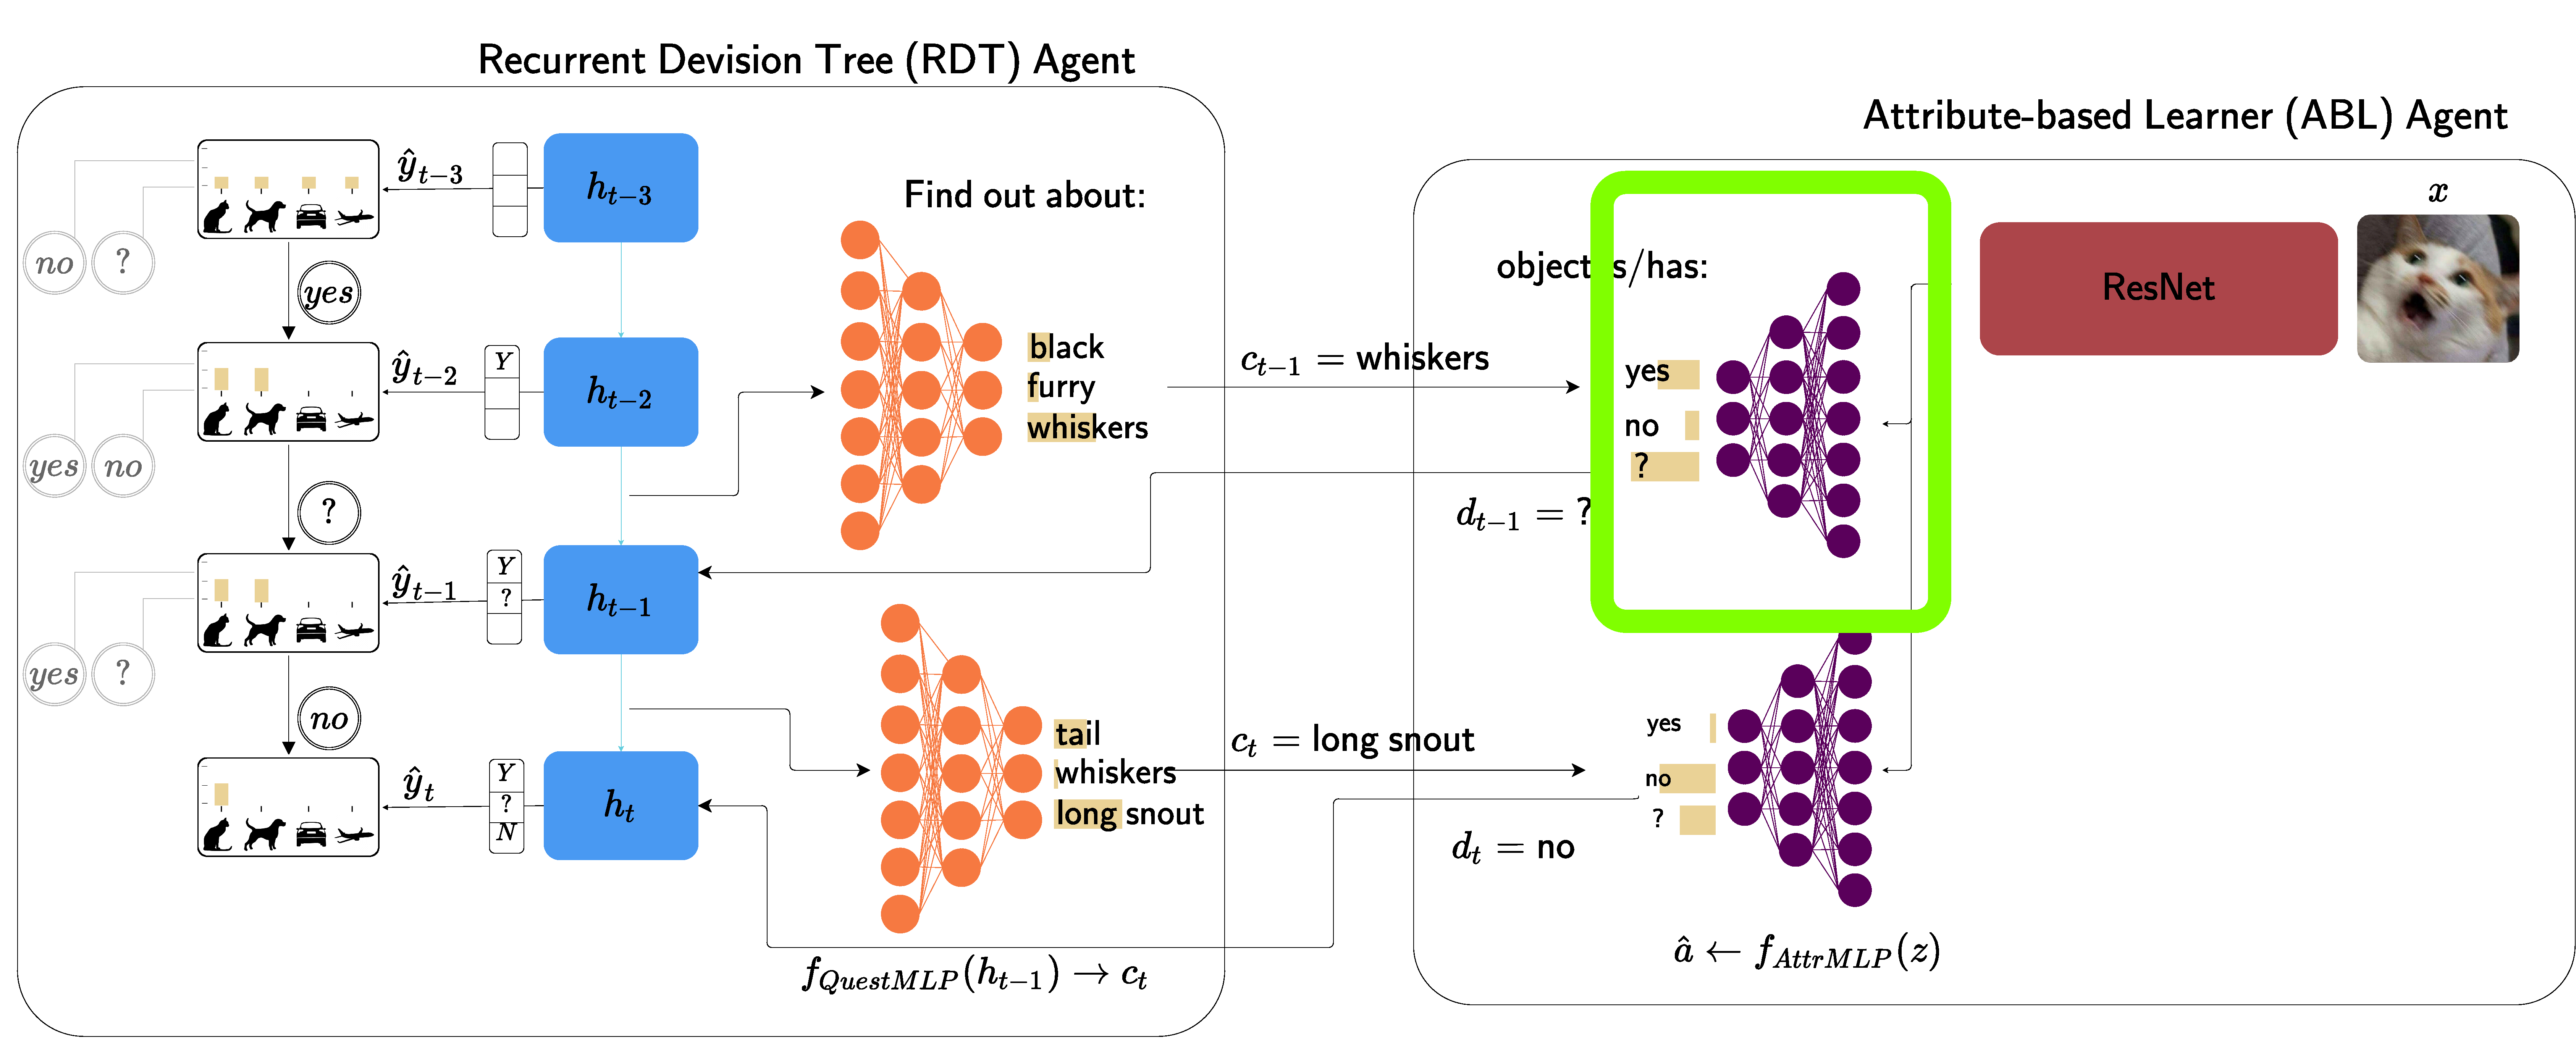
\includegraphics[width=0.8\textwidth]{images/where_is_uncertainty.pdf} 
\end{figure}
\begin{itemize}
	\item We use dropout uncertainty estimation to retrieve uncertainty (more on that later)
	\item We want the AbL to say 'I don't know in the case of high uncertainty
	\item However, we want to keep the ResNet as feature extractor
	\item Thus, we use dropout in $f_{AttrMLP}$ (more on that later)
	\item After extracting features, we do $n$ forward passes and compute variance
	\item This corresponds to model uncertainty
\end{itemize}
\end{frame}


\setbeamercolor{background canvas}{bg=white}
\setbeamercolor{normal text}{fg=darkgrey}
\usebeamercolor[fg]{normal text}
\setbeamertemplate{itemize item}{\color{darkgrey}$\circ$}	
\begin{frame}
\frametitle{Getting Uncertainty Information}
\framesubtitle{through dropout uncertainty information}
\begin{figure}
	\centering
	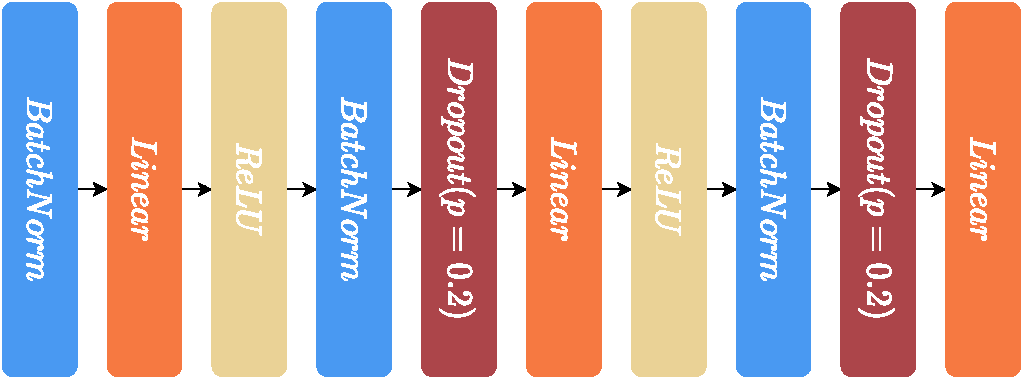
\includegraphics[width=0.7\textwidth]{images/f_attrMLP.pdf}
\end{figure}
\begin{itemize}
	\item We include dropout layers in our $f_{AttrMLP}$
	\item We tested different configurations and a combination of batchnorm and dropout worked best
\end{itemize}
\end{frame}



\setbeamercolor{background canvas}{fg=darkgrey}
\setbeamercolor{normal text}{fg=darkgrey}
\usebeamercolor[fg]{normal text}
\setbeamertemplate{itemize item}{\color{darkgrey}$\circ$}
\begin{frame}	
\frametitle{Using Uncertainty Information}
\framesubtitle{as an inductive bias}
\begin{itemize}
	\item Now, we have an uncertainty estimate
	\item But now, we need a way to use it
	\item we use two different strategies
	\begin{itemize}
		\item We prevent the model from asking questions regarding uncertain attributes $\rightarrow$ remRDTC
		\item We give the model the ability to answer with 'I don't know' as extended vocabulary $\rightarrow$ extRDTC
	\end{itemize}
	\item For both strategies, we need to make sure the model does not use any gradients coming from uncertain attributes
	\item This ensures that the uncertainty information only remains an inductive bias and the model does not misuse it
\end{itemize}
\end{frame}


\setbeamercolor{background canvas}{bg=white}	
\setbeamercolor{normal text}{fg=darkgrey}
\usebeamercolor[fg]{normal text}
\setbeamertemplate{itemize item}{\color{darkgrey}$\circ$}
\begin{frame}
\frametitle{Using Uncertainty Information}
\framesubtitle{Removing uncertain attributes}
\begin{figure}
	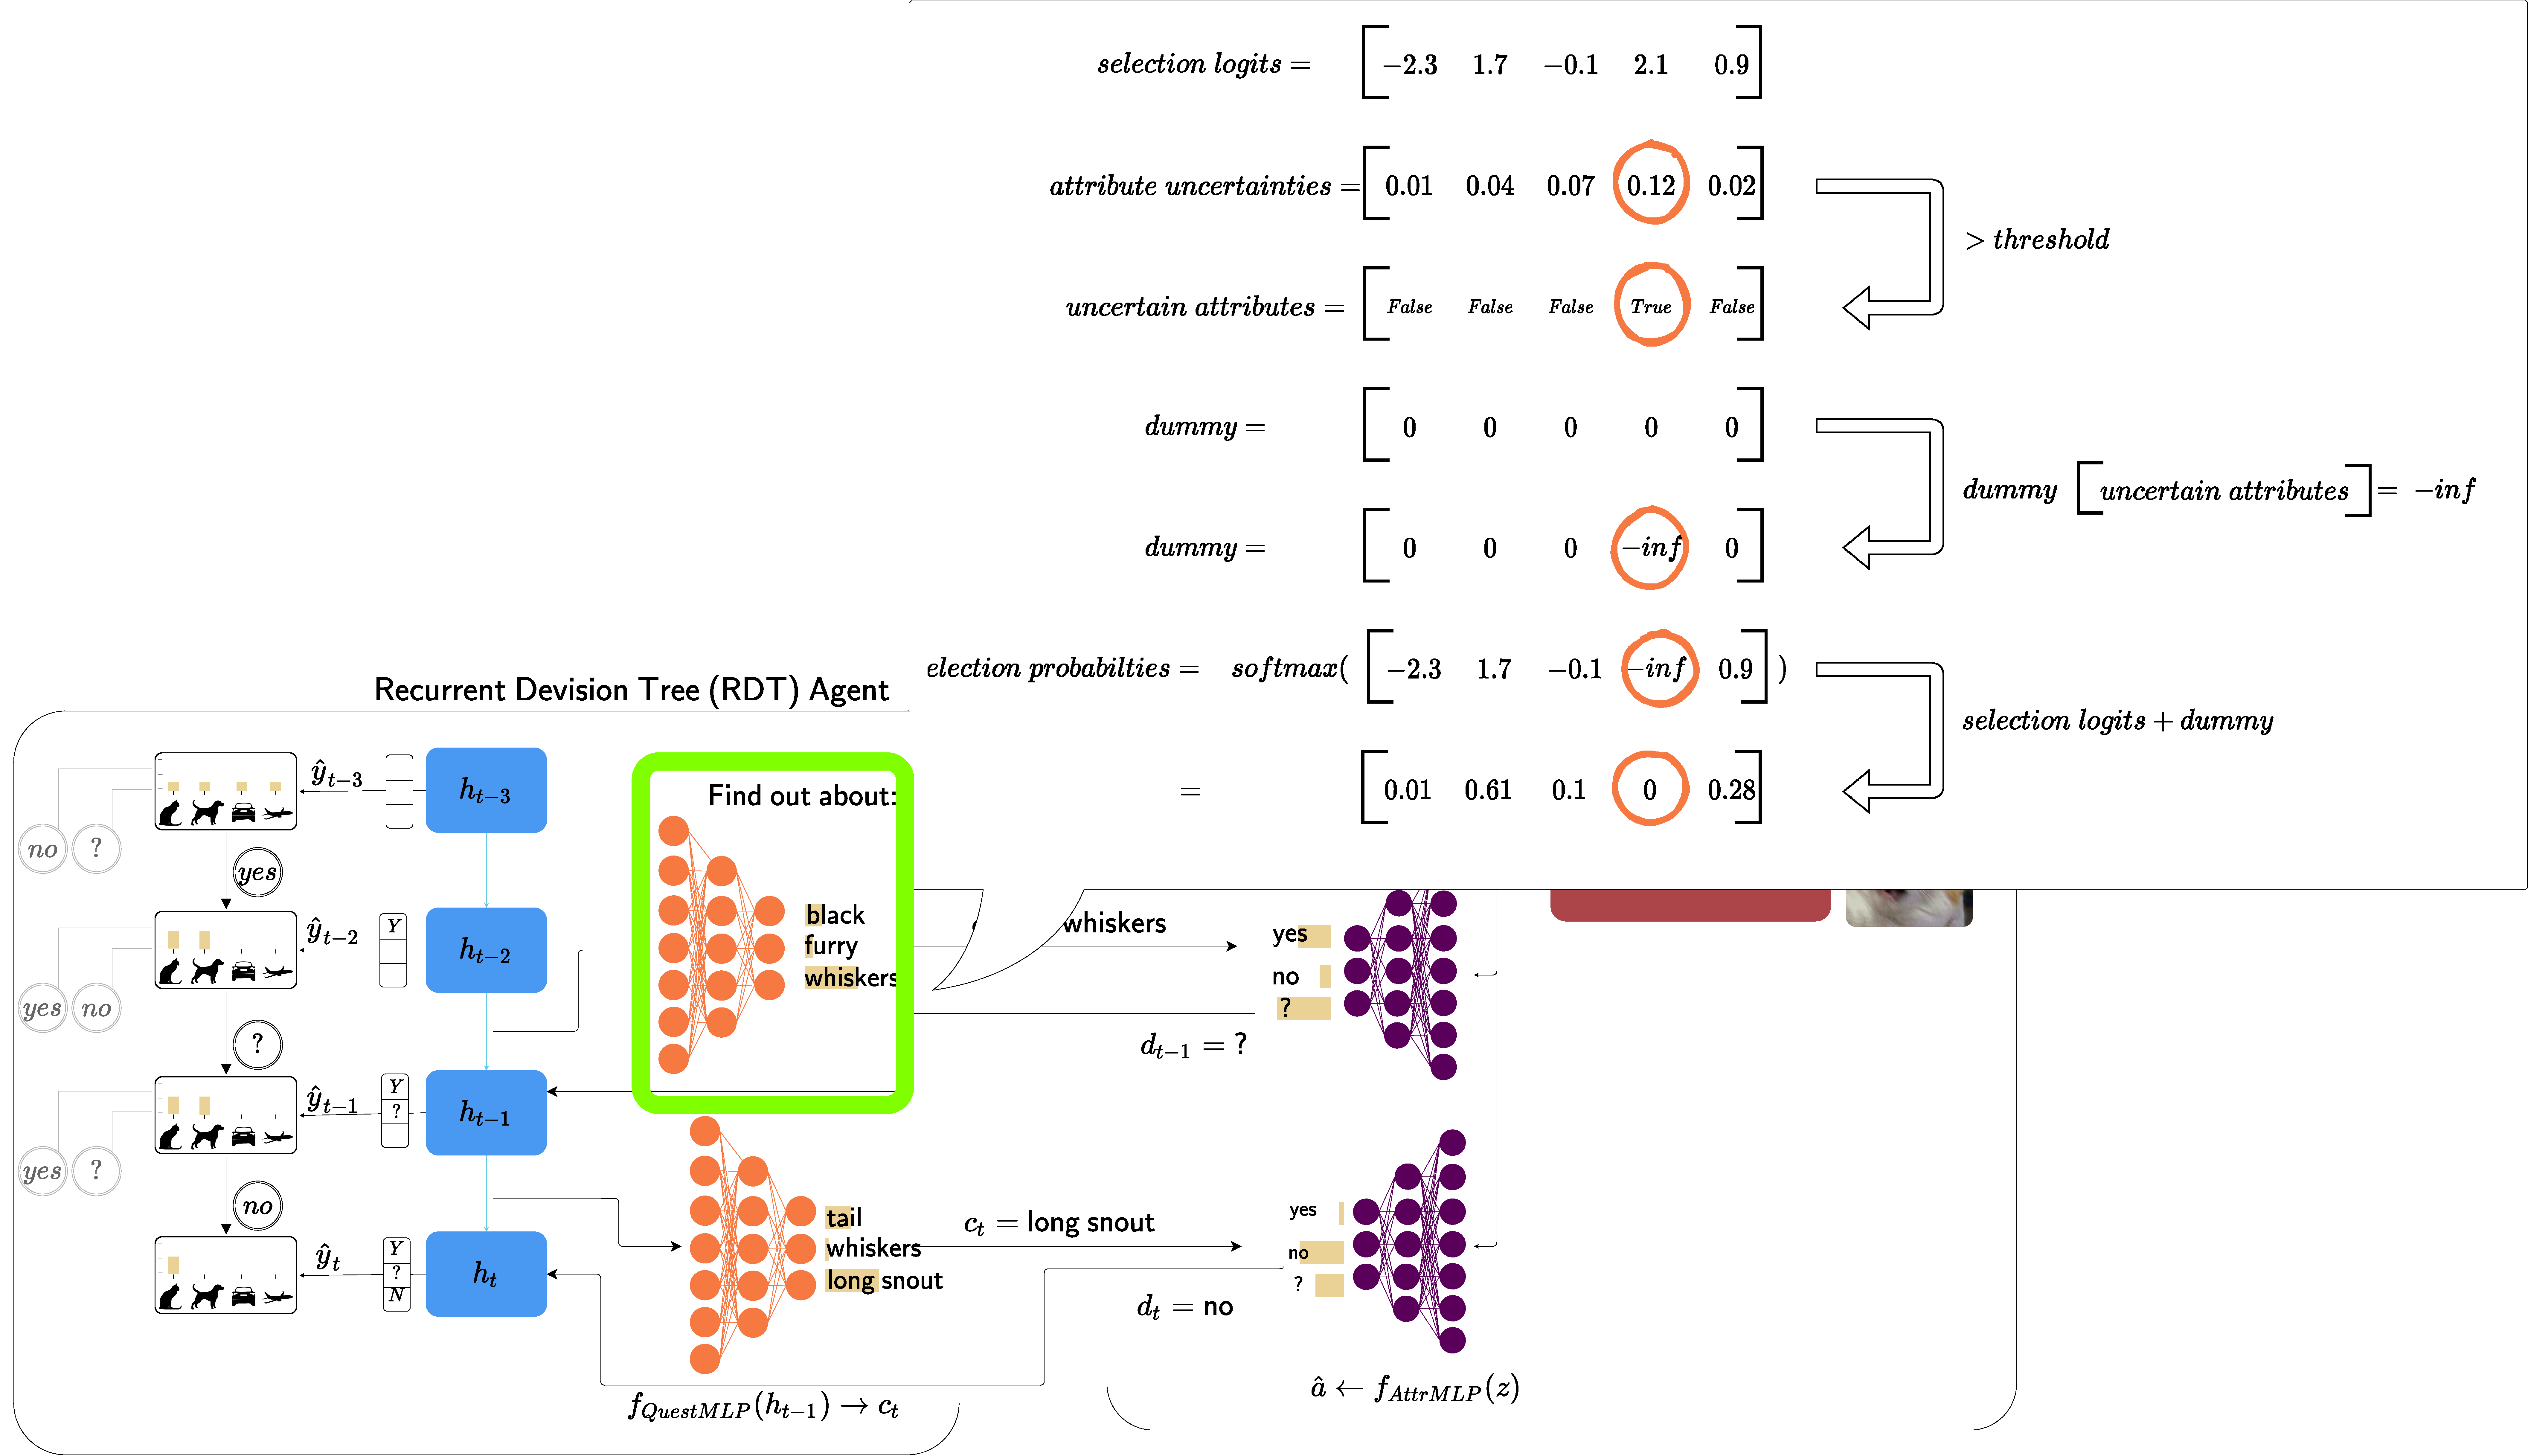
\includegraphics[width=0.8\linewidth]{images/how_to_remRDTC.png}
\end{figure}
\begin{itemize}
	\item The output from $f_{QuestMLP}$ is an index that indicates the attribute in question
	\item In case, an attribute is deemed uncertain by the AbL, we replace selection logits at those indices with $-\infty$
	This prevents the Gumbel softmax from picking such attributes as index
\end{itemize}
\end{frame}


\setbeamercolor{background canvas}{bg=white}
\setbeamercolor{normal text}{fg=darkgrey}
\usebeamercolor[fg]{normal text}
\setbeamertemplate{itemize item}{\color{darkgrey}$\circ$}	
\begin{frame}
\frametitle{Using Uncertainty Information}
\framesubtitle{Extending the vocabulary}
\begin{figure}
	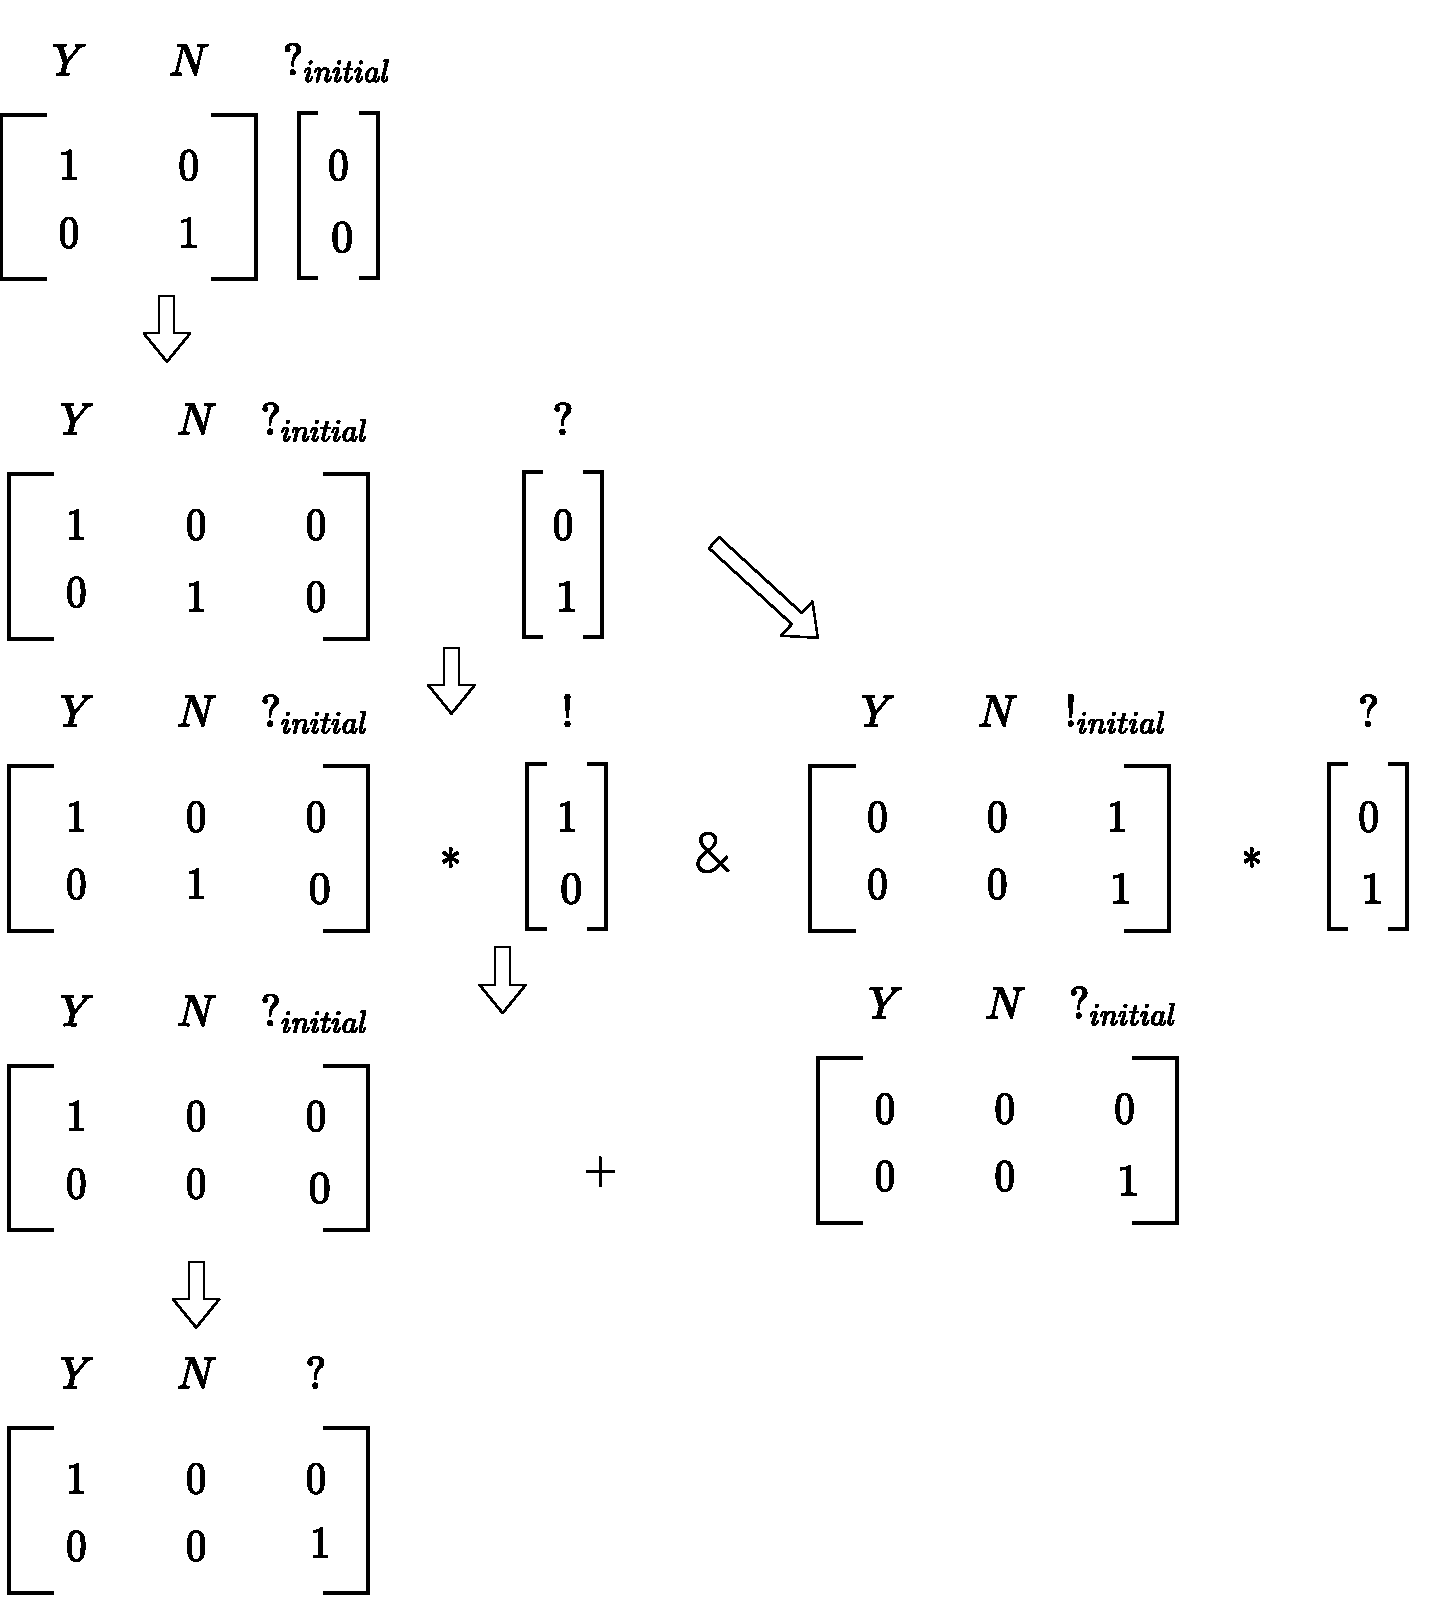
\includegraphics[width=0.6\linewidth]{images/extended_vocab.pdf}
\end{figure}
%\begin{itemize}
%	\item dsjf
%\end{itemize}
\end{frame}



\setbeamercolor{background canvas}{fg=darkgrey}	
\setbeamercolor{normal text}{fg=darkgrey}
\usebeamercolor[fg]{normal text}
\setbeamertemplate{itemize item}{\color{darkgrey}$\circ$}	
\begin{frame}
\frametitle{Using Uncertainty Information}
\framesubtitle{Extending the vocabulary}
\begin{figure}
	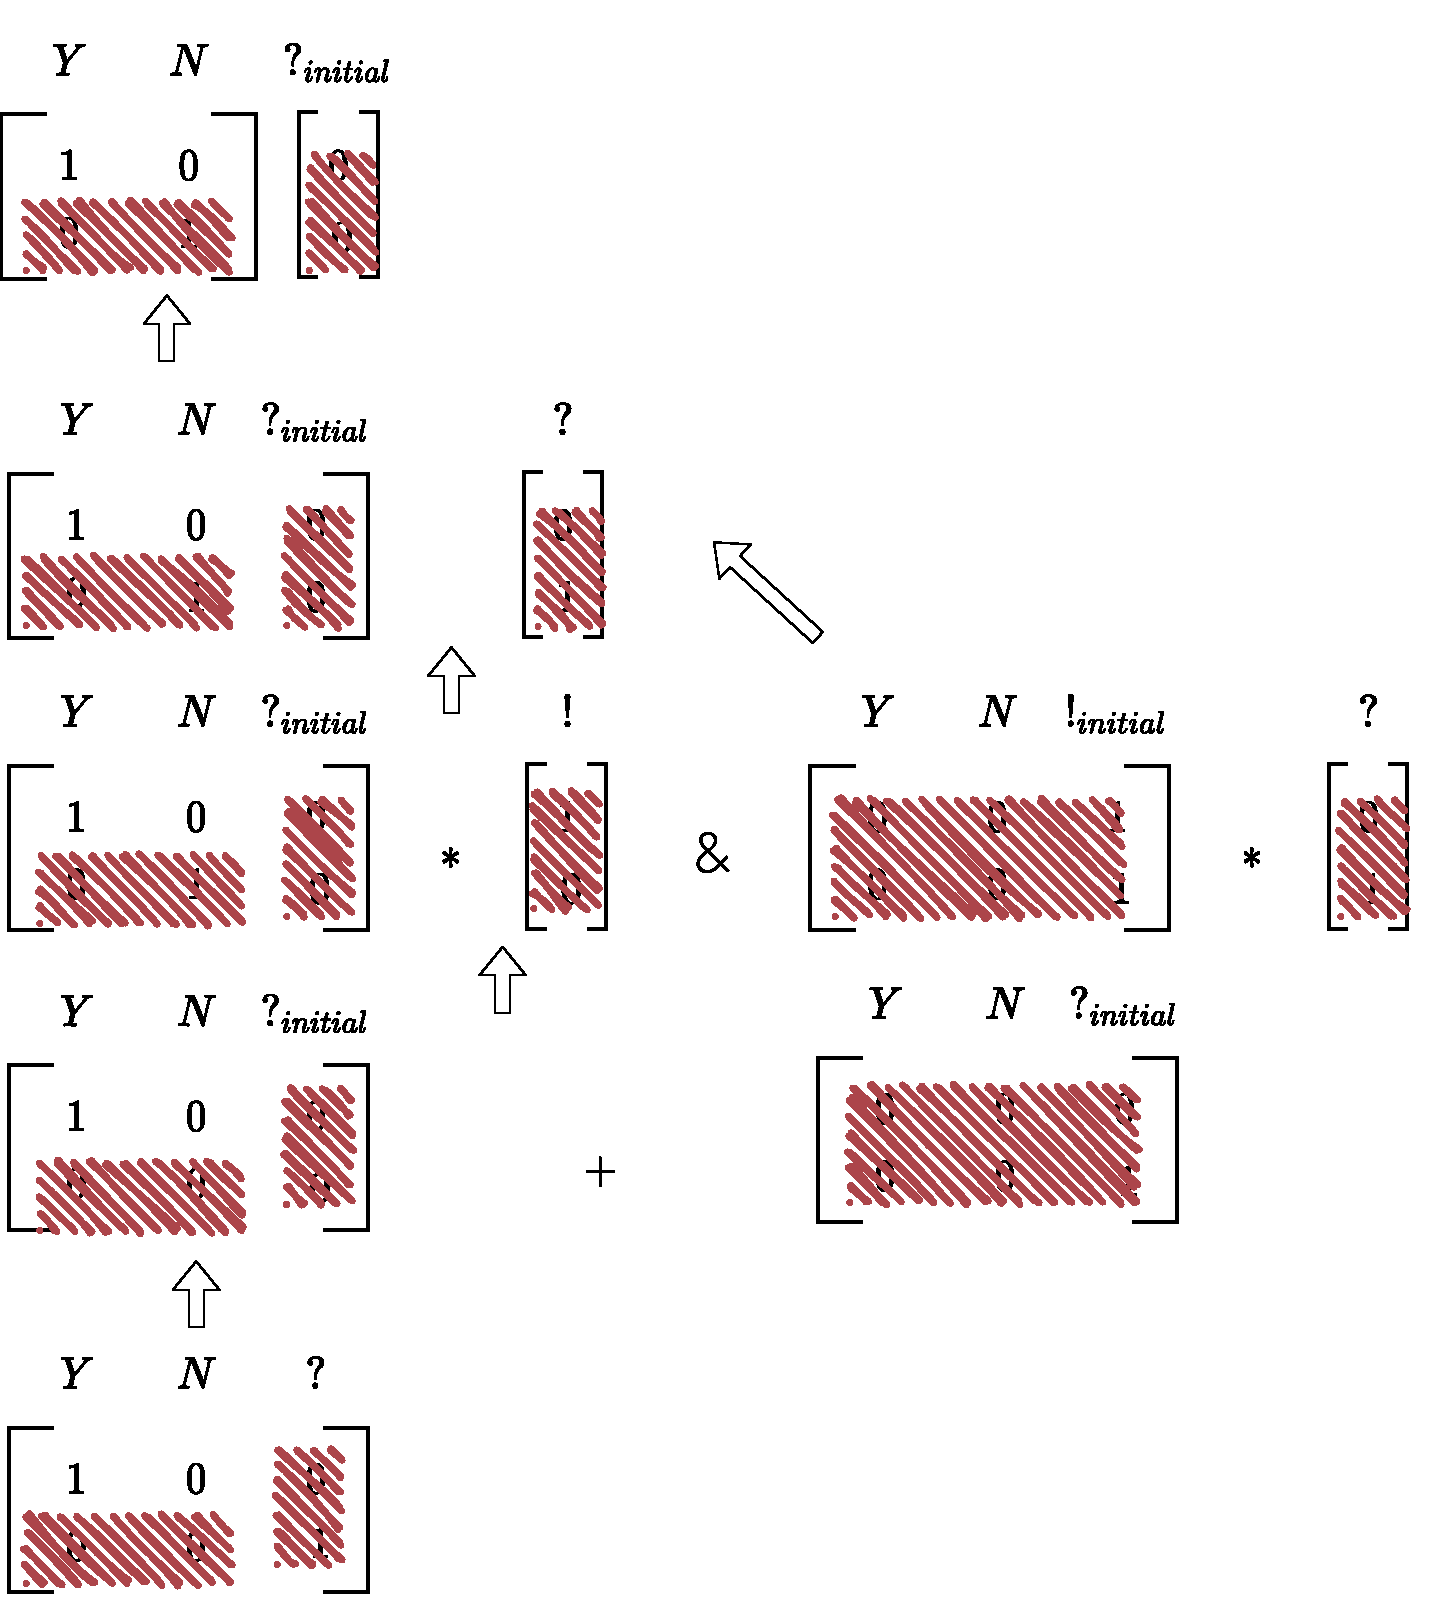
\includegraphics[width=0.6\linewidth]{images/extended_vocab_backward.pdf}
\end{figure}
%\begin{itemize}
%	\item dsjf
%\end{itemize}
\end{frame}



\setbeamercolor{background canvas}{bg=orange}
\setbeamercolor{normal text}{fg=white}	
\usebeamercolor[fg]{normal text}
\setbeamertemplate{itemize item}{\color{white}$\circ$}	
\begin{frame}[plain]{normal text}
\begin{itemize}
	\item We can interpret the variance arising from multiple forward passes in a dropout neural net as uncertainty
	\item We do this dropout uncertainty estimation in our $f_{AttrMLP}$
	\item We use the retrieved uncertainty estimate for either preventing the RDT from asking questions regarding uncertain attributes or extent the AbL's vocabulary
\end{itemize}
\end{frame}





% Experiments
\setbeamercolor{background canvas}{bg=white}
\setbeamercolor{normal text}{fg=darkgrey}
\usebeamercolor[fg]{normal text}
\setbeamertemplate{itemize item}{\color{darkgrey}$\circ$}
\begin{frame}
\frametitle{Experiments}
\framesubtitle{}
\begin{itemize}
	\item Now, we can make our model aware of, and express its uncertainties
	\item We use this in our experiments to:
	\begin{itemize}
		\item Investigate uncertainty and its relationship to other variables
		\item Test our model on OOD data
		\item Test the model's performance on benchmark datasets
	\end{itemize}
\end{itemize}
\end{frame}



\setbeamercolor{background canvas}{bg=white}
\setbeamercolor{normal text}{fg=darkgrey}
\usebeamercolor[fg]{normal text}
\setbeamertemplate{itemize item}{\color{darkgrey}$\circ$}	
\begin{frame}	
\frametitle{Experiments}
\framesubtitle{Investigating Uncertainties}
\begin{itemize}
	\item We investigate covariance of misclassification rate, uncertainty, and usage of attributes
\end{itemize} %TODO check whether this are correlations or covariances
	\begin{figure}
		\centering
		
\includegraphics[width=0.6\textwidth]{images/corr_matrix.pdf}
		%\caption{Correlations between misclassification rate, uncertainty, and usage of attributes.}
		%\label{fig:corr_matrix}
	\end{figure}
	\begin{itemize}
		\item Negative correlation between usage and misclassification rate
		\item Almost no correlation between uncertainty and misclassification rate
	\end{itemize}
\end{frame}




\setbeamercolor{background canvas}{bg=white}
\setbeamercolor{normal text}{fg=darkgrey}
\usebeamercolor[fg]{normal text}
\setbeamertemplate{itemize item}{\color{darkgrey}$\circ$}
\begin{frame}	
\frametitle{Experiments}
\framesubtitle{Investigating Uncertainties}
\begin{itemize}
	\item Let's have a look at the actual values
	\item Uncertainty and misclassification rate (usage is represented through size)
\end{itemize}
	\begin{figure}
		\centering
		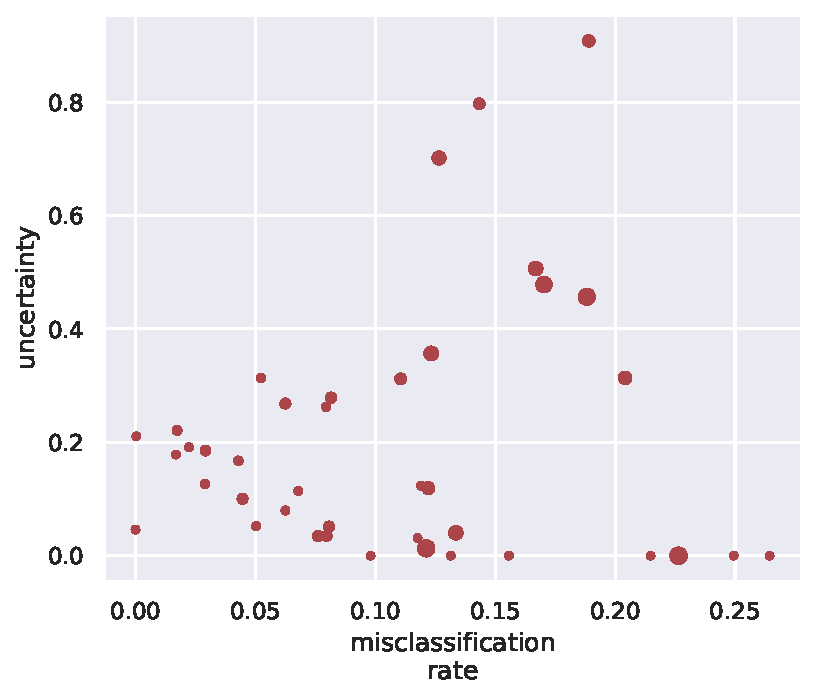
\includegraphics[width=0.6\textwidth]{images/error_sigma_corr_all.pdf} 
		%\caption{Misclassification rates of attributes and their respective uncertainties. The size of the points represents how often they are used.}
		%\label{fig:correlations}
	\end{figure}
	\begin{itemize}
		\item Uncertain attribute seem to be misclassified more often
	\end{itemize}
\end{frame} 



\setbeamercolor{background canvas}{bg=white}
\setbeamercolor{normal text}{fg=darkgrey}	
\usebeamercolor[fg]{normal text}
\setbeamertemplate{itemize item}{\color{darkgrey}$\circ$}	
\begin{frame}
\frametitle{Experiments}
\framesubtitle{OOD Detection}
\begin{itemize}
	\item We test extRDTC in a zero shot setting (using CUB dataset)
	\item A quarter of all classes were never seen during training
	\item We compare uncertainty values of seen and unseen classes
\end{itemize}
\begin{figure}
	\centering
	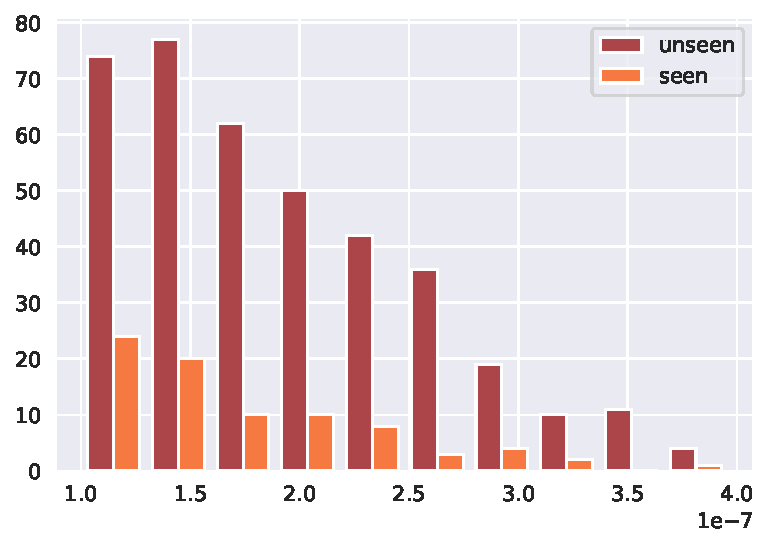
\includegraphics[width=0.6\textwidth]{images/zero_shot_class_uncertainty_median_hist.pdf}
	%\caption{Uncertainty values of attributes from seen and unseen classes. Examples from unseen classes have a higher attribute uncertainty. Attributes with an uncertainty value below $0.0000001$ are not shown.}
\end{figure}
\begin{itemize}
	\item Unseen classes have higher uncertainty values
\end{itemize}
\end{frame} 


\setbeamercolor{background canvas}{bg=white}
\setbeamercolor{normal text}{fg=darkgrey}
\usebeamercolor[fg]{normal text}
\setbeamertemplate{itemize item}{\color{darkgrey}$\circ$}	
\begin{frame}
\frametitle{Experiments}
\framesubtitle{Results on Benchmark Datasets}
\begin{table}
	\renewcommand{\arraystretch}{1.3}
	%\caption{We compare accuracy on AWA2, aPY, and CUB of our model and other methods. Standard deviations, denoted by $\pm$ are from five runs.}
	%\label{tab:benchmarks}
	\begin{tabular*}{\textwidth}{c @{\extracolsep{\fill}} c c c c}
		%\hline
		&                                AWA2&          aPY&          CUB\\
		\hline
		\hline
		ResNet \cite{he2016deep}&       98.2$\pm$ 0.0& 85.1$\pm$ 0.6 & 79.0$\pm$ 0.2 \\ 
		\hline 
		DT&                             78.0$\pm$ 0.4&64.3$\pm$ 0.6  & 19.3$\pm$ 0.3  \\ 
		\hline 
		dNDF\cite{kontschieder2015deep}&97.6$\pm$ 0.2&85.0$\pm$ 0.6 & 73.8$\pm$ 0.3 \\ 
		\hline 
		RDTC\cite{alaniz2019explainable}&98.0$\pm$ 0.1&85.7$\pm$ 0.7& 78.1$\pm$ 0.2   \\ 
		\hline 
		XDT&                            73.9$\pm$ 0.9&59.9$\pm$ 1.5  & 4.9$\pm$ 1.3 \\ 
		\hline 
		aRDTC\cite{alaniz2019explainable}&98.6&         86.1&  77.9$\pm$ 0.6\\ 
		\hline
		remRDTC(ours)&          98.7          &          86.4&  77.7\\ 
		\hline
		extRDTC(ours)&          98.7          &          85.4&  77.8\\
		%\hline 
	\end{tabular*}
\end{table}
\end{frame} 



\setbeamercolor{background canvas}{bg=white}
\setbeamercolor{normal text}{fg=darkgrey}
\usebeamercolor[fg]{normal text}
\setbeamertemplate{itemize item}{\color{darkgrey}$\circ$}	
\begin{frame}
\frametitle{Experiments}
\framesubtitle{Results on Benchmark Datasets}
\begin{table}
		\begin{tabular*}{\textwidth}{c  @{\extracolsep{\fill}}c c c c}
		& aRDTC \cite{alaniz2019explainable} & Random Baseline & remRDTC & extRDTC \\ 
		%\hline 
		%\hline
		\textbf{AWA2}& & & &\\\hline\hline
		Class &  98.6&  98.5&  98.7&  98.7\\ 
		\hline 
		Attribute & 80.4 & 84.6 &  87.5&  82.31\\ 
		&  &  &  &  \\
		\textbf{aPY}& & & &\\\hline\hline
		Class & 86.1&  86.5&  86.4&  85.4\\ 
		\hline 
		Attribute &  86.4&  86.2&  87.6& 87.12 \\ 
		&  &  &  &  \\ 
		\textbf{CUB}& & & &\\\hline\hline
		Class &  77.9& 76.8 & 77.7 & 77.8 \\ 
		\hline
		Attribute &  68.6&  70.0& 77.4 & 82.6 \\ 
		&  &  &  &  \\ 
	\end{tabular*}
\end{table}
\end{frame} 



\setbeamercolor{background canvas}{bg=orange}
\setbeamercolor{normal text}{fg=white}
\usebeamercolor[fg]{normal text}
\setbeamertemplate{itemize item}{\color{white}$\circ$}
\begin{frame}[plain]
\begin{itemize}
	\item We have seen that the RDTC uses only a small set of attributes that it rarely misclassifies
	\item Unseen classes yield higher uncertainty
	\item Both our proposed strategies perform well on benchmark datasets
\end{itemize}
\end{frame}
%\setbeamertemplate{background canvas}{bg=white}

\setbeamercolor{background canvas}{bg=white}
\setbeamercolor{normal text}{fg=darkgrey}
\usebeamercolor[fg]{normal text}
\setbeamertemplate{itemize item}{\color{darkgrey}$\circ$}	
\begin{frame}
\frametitle{Discussion}
\framesubtitle{Looking back...}
\begin{itemize}
	\item The right kind of uncertainty?
	\begin{itemize}
		\item We only consider model uncertainty (epistemic uncertainty)
		\item Uncertainty arising from noise or occlusions in the data is not considered
	\end{itemize}
	\item Uncertainty versus risk
	\begin{itemize}
		\item The variance we view as uncertainty is often called 'risk' in decision theory
	\end{itemize}
	\item Beyond attribute uncertainty
	\begin{itemize}
		\item Estimate uncertainty in other parts as the model (i.e. $f_{ClassMLP}$)
	\end{itemize}
\end{itemize}

\end{frame} 










% Conclusion
\setbeamercolor{background canvas}{bg=white}
\setbeamercolor{normal text}{fg=darkgrey}
\usebeamercolor[fg]{normal text}
\setbeamertemplate{itemize item}{\color{darkgrey}$\circ$}
\begin{frame}
\frametitle{Conclusions}
\framesubtitle{A qualitative Example}
\begin{figure}
	\centering
	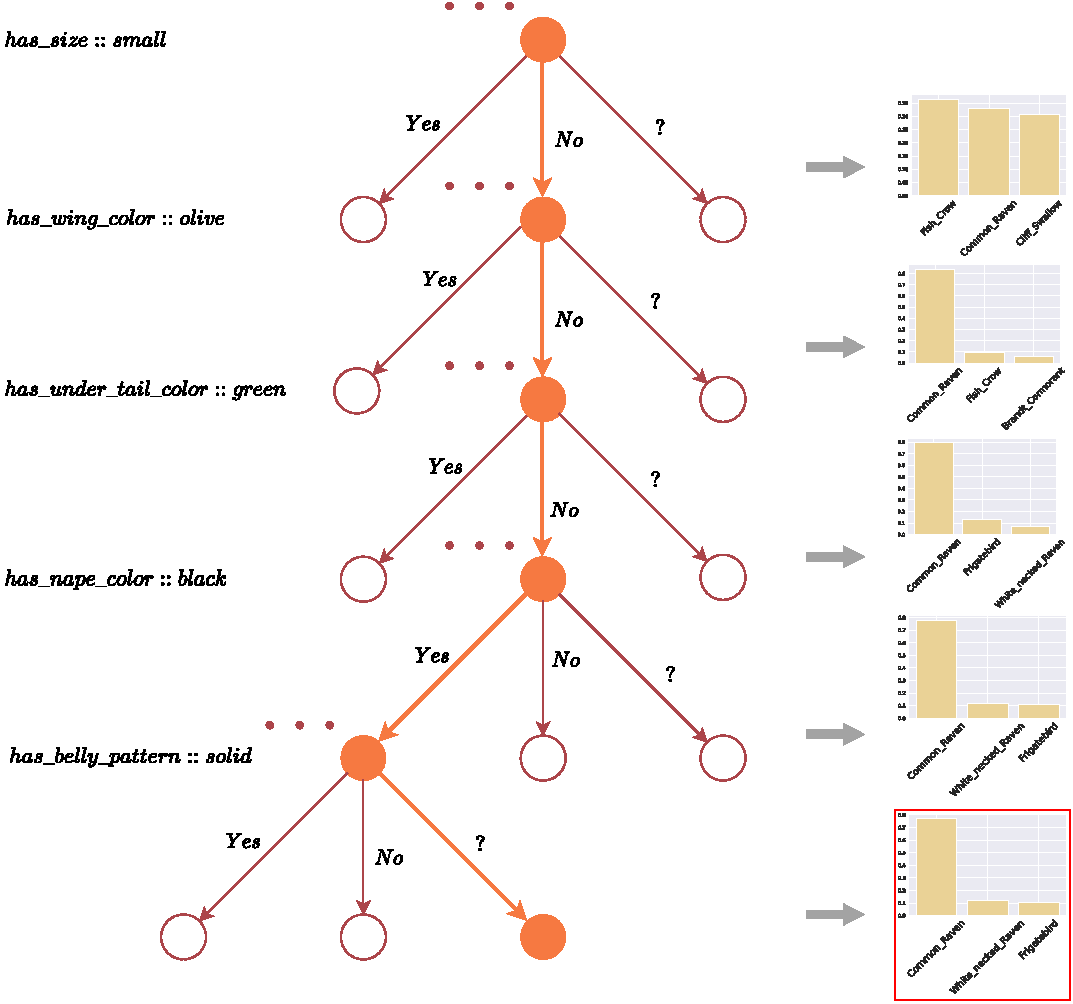
\includegraphics[width=0.7\textwidth]{images/example_tree.pdf}
%\caption{Five steps of a extRDTC decision process. The model has used an uncertain attribute and the final classification is wrong. In such a case, a human user could be consulted and manually classify the image. Note that the the softmax classification output is highly confident despite being wrong.}
\label{fig:example_tree}
\end{figure}
\end{frame} 







\setbeamercolor{background canvas}{bg=orange}
\setbeamercolor{normal text}{fg=white}
\usebeamercolor[fg]{normal text}
\setbeamertemplate{itemize item}{\color{white}$\circ$}
\begin{frame}
\frametitle{Conclusions}
%\framesubtitle{}
\begin{itemize}
	\item We estimate uncertainty in the RDTC model
	\item This uncertainty is used in the remRDTC and extRDTC strategies
	\item We investigate uncertainty and its relationship to other variables
	\item We show that OOD examples yield high uncertainty
	\item The RDTC models using uncertainty information achieve state of the art accuracy on benchmark image classification tasks
\end{itemize}
\end{frame}




\setbeamercolor{background canvas}{bg=white}
\setbeamercolor{normal text}{fg=darkgrey}
\usebeamercolor[fg]{normal text}
\setbeamertemplate{itemize item}{\color{darkgrey}$\circ$}
\begin{frame}
	\bibliographystyle{alpha}
	\bibliography{bibliography}
\end{frame}


\end{document}
